\section{Spínací jednotka}
\begin{figure}[H]
   \centering
   \def\svgwidth{0.4\columnwidth}
   \input{images/svg/otopna-soustava/vyrez-spinaci-jednotka.pdf_tex}
    \caption[Umístění spínacích jednotek.]{Výřez z obrázku \ref{fig:otopna-soustava-a-elektronika-rez-domu} – spínací jednotky.}
    \label{fig:vyrez-spinaci-jednotka}
\end{figure}
Na obrázku \ref{fig:vyrez-spinaci-jednotka} je výřez části z celkového nákresu (obrázek \ref{fig:otopna-soustava-a-elektronika-rez-domu}) pro spínací jednotky. Pro spínání čerpadel a signalizačních LED slouží dva zakoupené relé moduly po čtyřech kanálech \cite{rele-modul-informace}. Relé umožňují spínat výkony 250 VAC při max. 10~A a 30 V DC při max. 10~A. Jednotlivé kanály jsou oddělené galvanicky (dále je vyfrézovaná část DPS mezi výkonovou částí a spínací částí), též je možné využít různých zdrojů pro napájení spínací části a napájení relé. Zapojení jednoho kanálu je v příloze \ref{app:schemata-ostatni}. Celý relé modul je na obrázku \ref{fig:ctyr-kanalovy-rele-modul}. Pro spínání síťového napětí je použit jeden relé modul, pro spínání slaboproudého napětí (LED diody, kotel) je použit druhý relé modul.

%\begin{figure}[H]
%    \centering
%    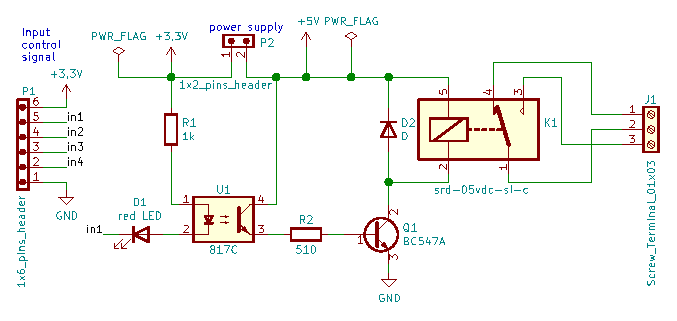
\includegraphics[width=\textwidth]{images/svg/kicad/rele-modul-jeden-kanal.eps}
%    \caption{Zapojení jednoho kanálu relé modulu.}
%    \label{fig:rele-modul-jeden-kanal}
%\end{figure}


\begin{figure}[H]
    \centering
    \includegraphics[width=0.5\textwidth]{images/ctyr-kanalovy-rele-modul.png}
    \caption[Čtyřkanálový relé modul.]{Čtyřkanálový relé modul \cite{ctyr-kanalovy-rele-modul}.}
    \label{fig:ctyr-kanalovy-rele-modul}
\end{figure}